\documentclass[aspectratio=169]{beamer}
\usepackage[T1]{fontenc} \usepackage{lmodern} \usepackage[utf8]{inputenc}
\usepackage[english]{babel} \usepackage{booktabs}
\usepackage{graphicx,subcaption} \usepackage{amssymb,amsmath}
\graphicspath{{figures/}}
\usepackage[citestyle=authoryear,bibstyle=authoryear,backend=biber,url=false,doi=false,isbn=false]{biblatex} \bibliography{refs}
\usepackage{hyperref}

% Make Adobe Reader use the RGB rendering model for pages with transparency.
\pdfpageattr{/Group << /S /Transparency /I true /CS /DeviceRGB>>}

\mode<presentation>{
	\usetheme{Malmoe}
	\usecolortheme{beaver}
	\setbeamertemplate{footline}[page number]
	\setbeamertemplate{navigation symbols}{}
}

%------------------------------------------------

\DeclareMathOperator*{\diag}{diag}
\DeclareMathOperator*{\argmin}{arg\,min}
\DeclareMathOperator*{\spn}{span}
\newcommand{\G}{\mathcal{G}}
\newcommand{\V}{\mathcal{V}}
\newcommand{\E}{\mathcal{E}}
\newcommand{\bO}{\mathcal{O}}
\newcommand{\R}{\mathbb{R}}

\newcommand{\good}[1]{{\color[rgb]{0.2,0.6,0.2}#1}}
\newcommand{\bad}[1]{{\color{red}#1}}
\newcommand{\txt}[1]{\hspace{.5cm} \text{#1} \hspace{.5cm}}
\newcommand{\define}[1]{\item{\usebeamercolor[fg]{enumerate item}#1}:}
\newcommand{\HRule}{{\usebeamercolor[bg]{subsection in head/foot} \rule{\linewidth}{0.5mm}}}

%------------------------------------------------

\begin{document}

\begin{frame}[plain]
	%\titlepage
	\begin{center}

		\begin{minipage}{0.7\linewidth}
			\textsc{\large A Network Tour of Data Science}
		\end{minipage}
		\hfill
		\begin{minipage}{0.25\linewidth}
			
\includegraphics[width=\linewidth]{logo_epfl}
		\end{minipage}
		\vspace{0.5cm}

		\HRule
		\vspace{0.55cm}
		{
			\usebeamercolor[fg]{frametitle}
			\textsc{\Large Practical Informations}\\
			%\textsc{\Large Lab Sessions}\\
			%\textsc{\Large Laboratories}\\
			\vspace{0.3cm}
		}
		\HRule
		\vspace{0.8cm}

		\hspace{0.5cm}
		\begin{minipage}{0.4\linewidth}
			\footnotesize
			\textbf{Teachers} \\
			Pierre \textsc{Vandergheynst} \\
			Pascal \textsc{Frossard} \\
		\end{minipage}
		\begin{minipage}{0.4\linewidth}
			\footnotesize
			\textbf{Assistants} \\
			Michaël \textsc{Defferrard} \\
			Effrosyni \textsc{Simou} \\
			Hermina \textsc{Petric Maretić} \\
			Rodrigo \textsc{Pena} \\
			Eda \textsc{Bayram} \\
			Benjamin \textsc{Ricaud} \\
		\end{minipage}

		\vspace{0.4cm}
		{\footnotesize EPFL LTS2 \& LTS4 laboratories
		\hfill September 18, 2018}

	\end{center}
\end{frame}

%------------------------------------------------

\begin{frame}
	\frametitle{Team}
	\begin{figure}
		\centering
		\captionsetup{justification=centering}
		\begin{subfigure}[b]{0.14\linewidth}
			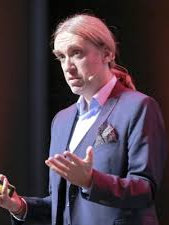
\includegraphics[width=\linewidth]{picture_pierre}
			\caption*{Pierre\\Vandergheynst}
		\end{subfigure}
		\hfill
		\begin{subfigure}[b]{0.14\linewidth}
			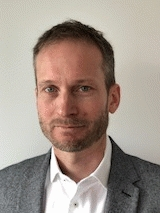
\includegraphics[width=\linewidth]{picture_pascal}
			\caption*{Pascal\\Frossard}
		\end{subfigure}
		\hfill
		\begin{subfigure}[b]{0.14\linewidth}
			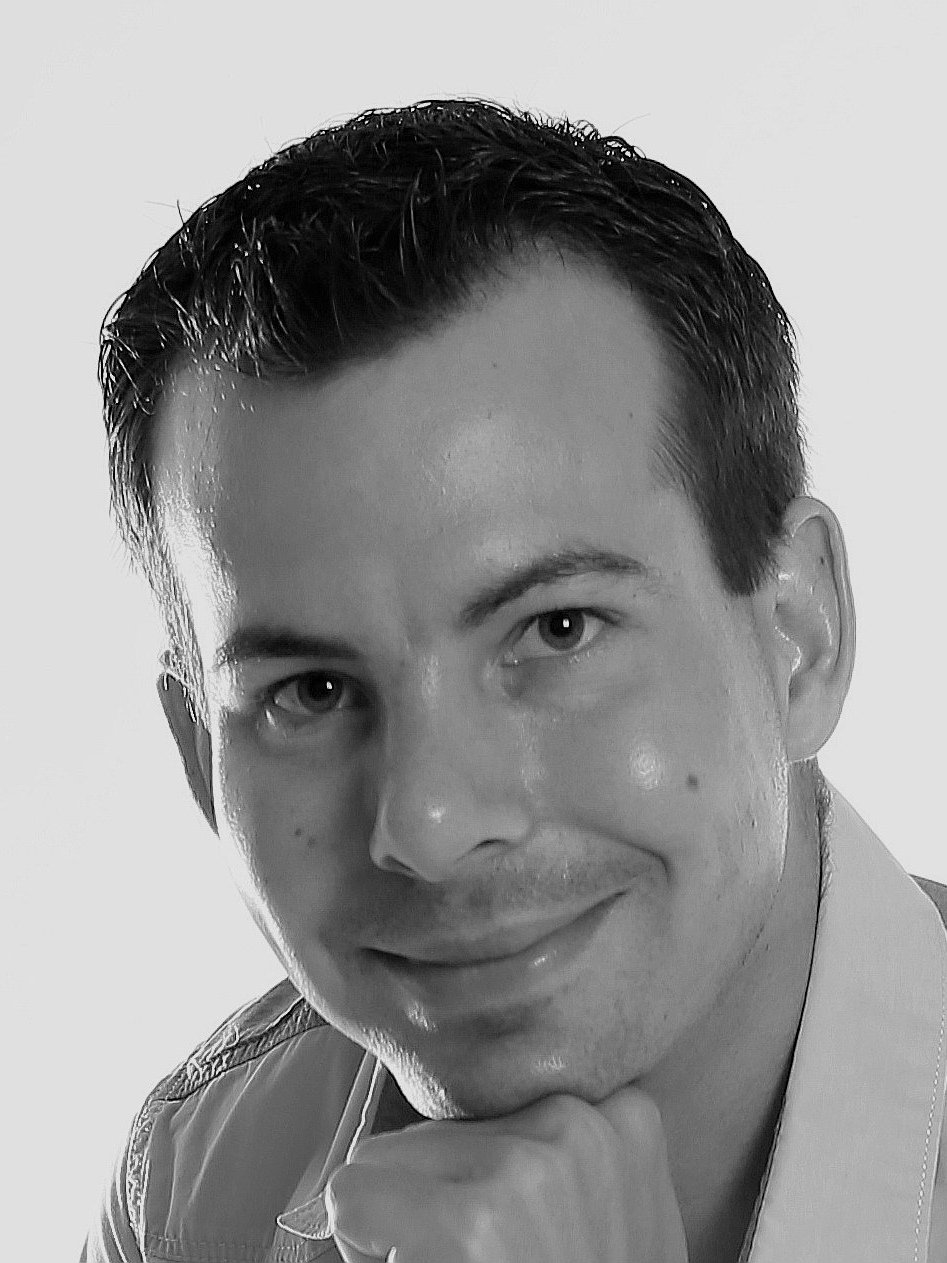
\includegraphics[width=\linewidth]{picture_michael}
			\caption*{Michaël\\Defferrard}
		\end{subfigure}
		\hfill
		\begin{subfigure}[b]{0.14\linewidth}
			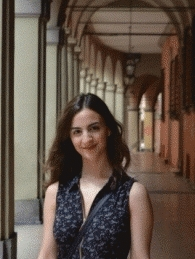
\includegraphics[width=\linewidth]{picture_ersi}
			\caption*{Effrosyni\\Simou}
		\end{subfigure}
		\\
		\vspace{1em}
		\begin{subfigure}[b]{0.14\linewidth}
			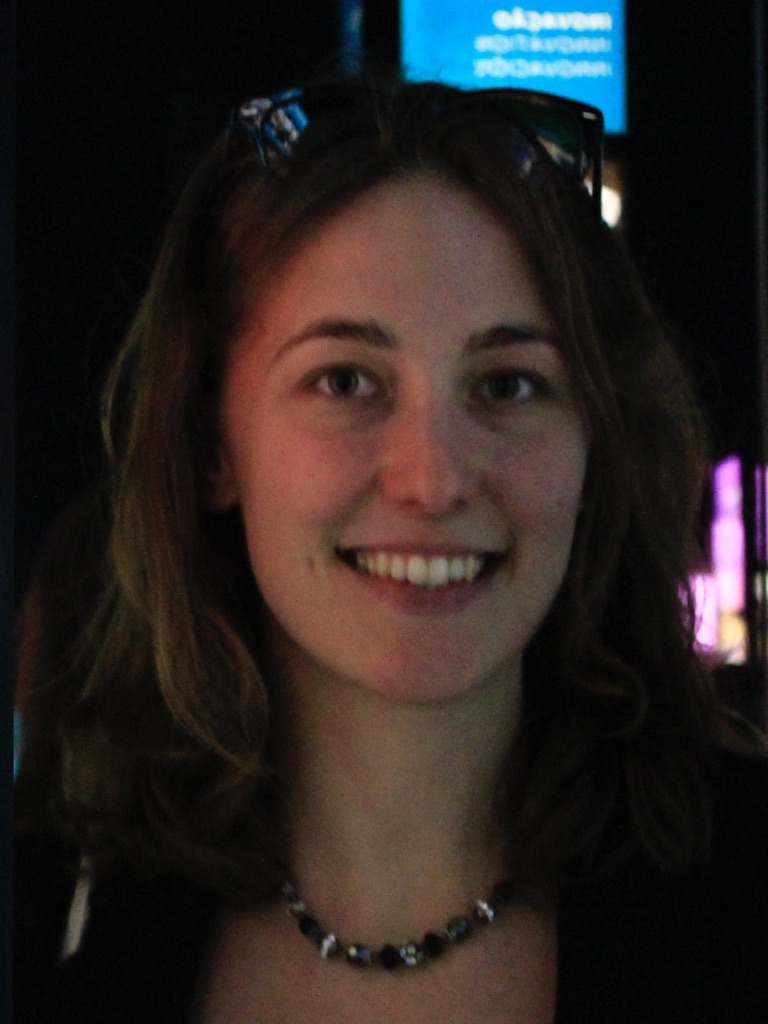
\includegraphics[width=\linewidth]{picture_hermina}
			\caption*{Hermina\\Petric Maretić}
		\end{subfigure}
		\hfill
		\begin{subfigure}[b]{0.14\linewidth}
			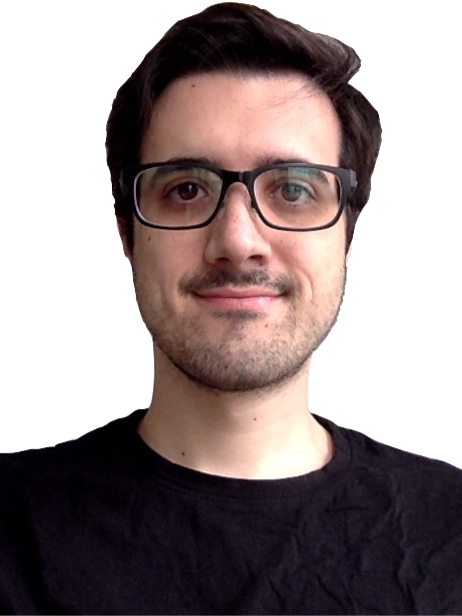
\includegraphics[width=\linewidth]{picture_rodrigo}
			\caption*{Rodrigo\\Pena}
		\end{subfigure}
		\hfill
		\begin{subfigure}[b]{0.14\linewidth}
			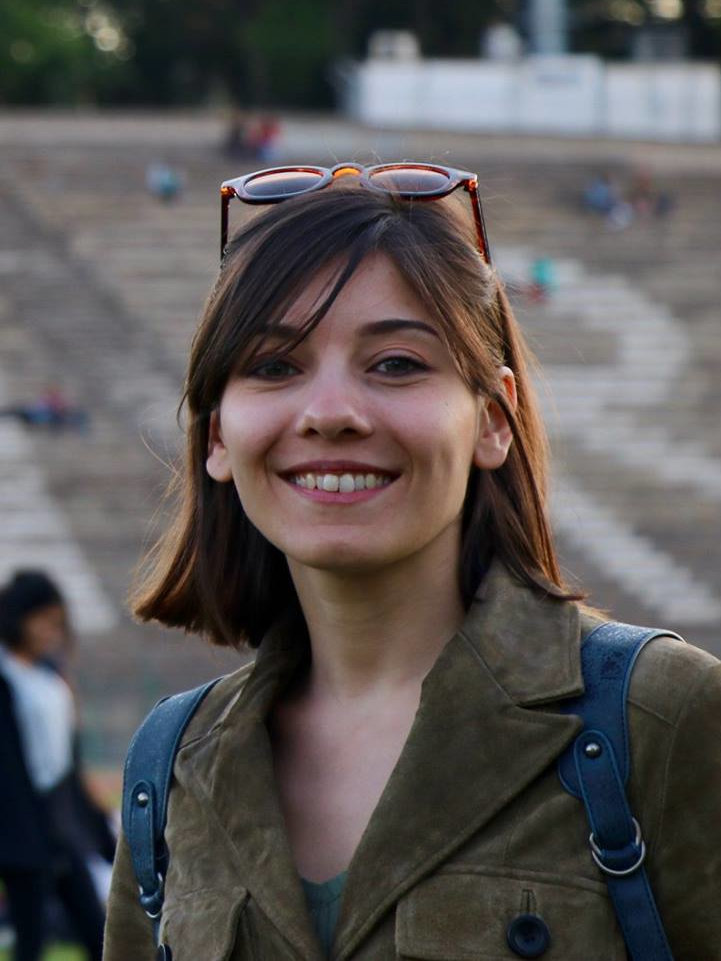
\includegraphics[width=\linewidth]{picture_eda}
			\caption*{Eda\\Bayram}
		\end{subfigure}
		\hfill
		\begin{subfigure}[b]{0.14\linewidth}
			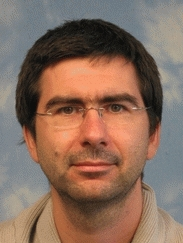
\includegraphics[width=\linewidth]{picture_benjamin}
			\caption*{Benjamin\\Ricaud}
		\end{subfigure}
	\end{figure}
\end{frame}

%------------------------------------------------

\begin{frame}
	\frametitle{Enrollment}
	% Poll: from which section are you from.
	\centering
	\includegraphics[width=0.9\linewidth]{enrollment}
\end{frame}

%------------------------------------------------

\begin{frame}
	\frametitle{Content: \textbf{A Network Tour} of Data Science}
	% First networks alone. Then data on networks.
	\begin{minipage}{0.4\linewidth}
		\begin{enumerate}
			\item Network Science
			\vspace{2em}
			\item Spectral Graph Theory
			\vspace{2em}
			\item Graph Signal Processing
			\vspace{2em}
			\item Machine Learning
		\end{enumerate}
	\end{minipage}
	\hfill
	\begin{minipage}{0.57\linewidth}
		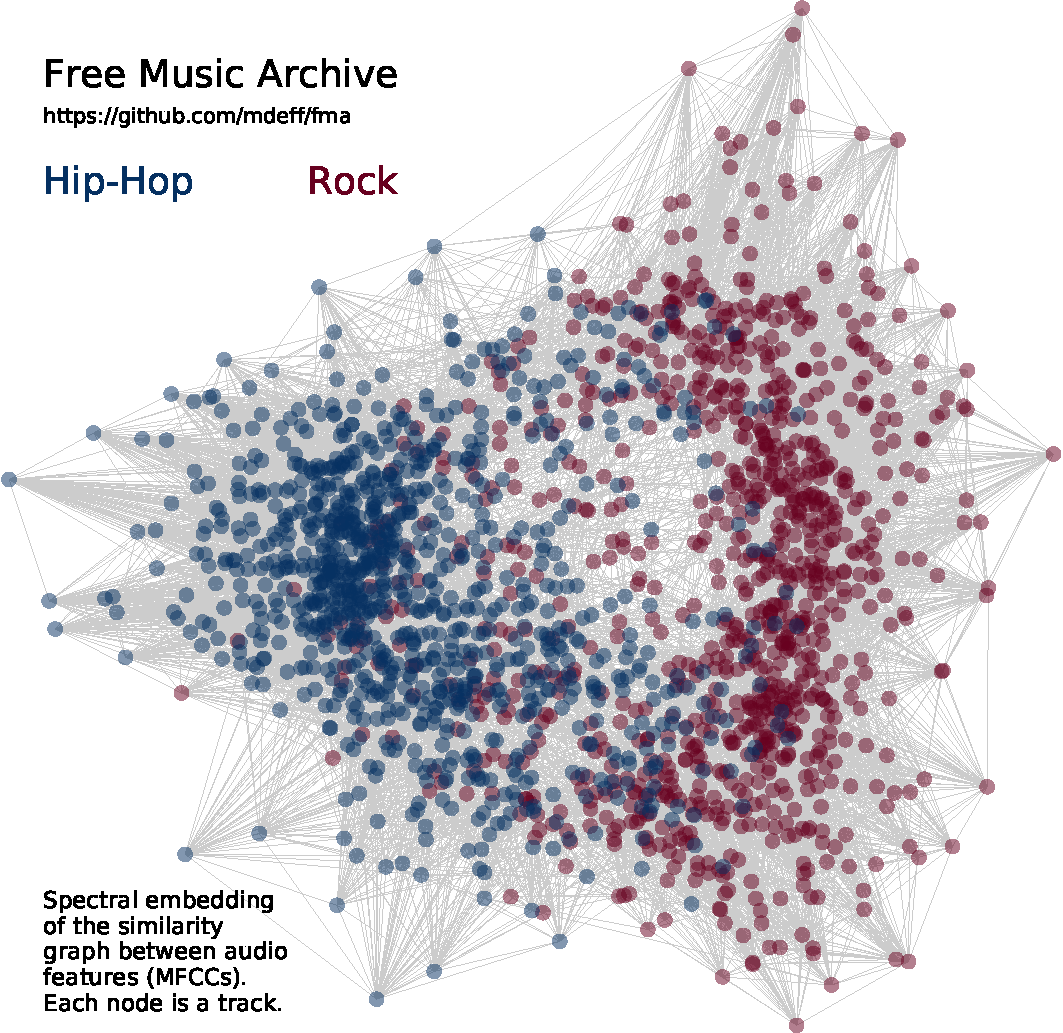
\includegraphics[width=\linewidth]{fma_illustration}
	\end{minipage}
\end{frame}

%------------------------------------------------

\begin{frame}
	\frametitle{Content: A Network Tour \textbf{of Data Science}}
	\begin{figure}
		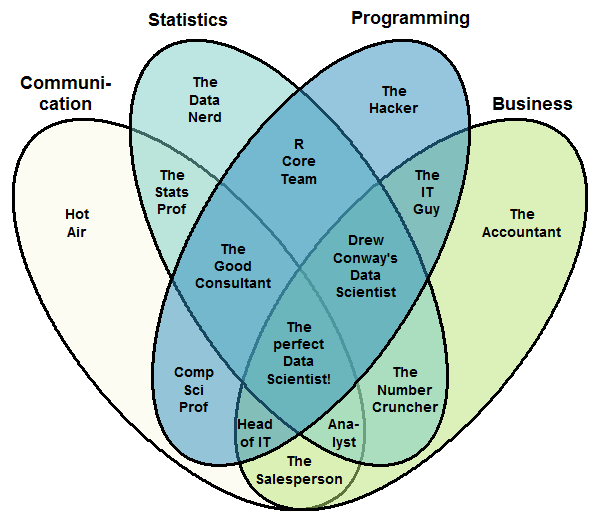
\includegraphics[height=0.85\textheight]{data_scientist}
	\end{figure}
\end{frame}

%------------------------------------------------

\begin{frame}
	\frametitle{Evaluation}
	Joint evaluation of theoretical and practical skills through a project.
	\vfill
	Two parts:
	\begin{enumerate}
		\item Guided with four milestones that follow the lectures.
		\item Open ended extra work (e.g., changing the graph, adding features, exploring other algorithms, gathering complementary data).
	\end{enumerate}
	\vfill
	Grading:
	\begin{itemize}
		\item 50\% for acquiring the course material in a structured way.
		\item 50\% for being creative and able to understand data, i.e., Data Science.
	\end{itemize}
\end{frame}

%------------------------------------------------

\begin{frame}
	\frametitle{Project flow}
	% milestones are mandatory
	% you might omit their content in the report and presentation if it doesn't fit your story
	% your solution, using the theory seen in class and the practical skills trained during labs.
	\begin{enumerate}
		\item Form teams of four and choose a project from a list of ten. Register on Moodle.
		\vfill
	\item Complete and handle (on Moodle) the four milestones (Jupyter notebooks).
		\vfill
		\item Work on the open ended extension.
		\vfill
	\item Write and handle (on Moodle) a coherent 5 pages PDF report that tells a data story.
		\vfill
		\item Handle all the code produced for the project as a git repository. On GitHub, with a proper readme, license, etc.
		\vfill
		\item Impress us in a presentation! Presentation of 15 minutes in front of the class.
	\end{enumerate}
\end{frame}

%------------------------------------------------

\begin{frame}
	\frametitle{Milestones}
	\begin{enumerate}
		\item Template notebook with instructions given on GitHub.
		\item Around two weeks to complete.
		\item At least one lab session to ask questions.
		\item Completed notebook to be handled on Moodle.
		\item Solutions posted on GitHub.
		\item Grades given on Moodle.
	\end{enumerate}
	\vfill
	Four topics that follow the lectures, with a Data Science taint:
	\begin{enumerate}
		\item Network properties
		\item Network models
		\item Spectral Graph Theory
		\item Graph Signal Processing
	\end{enumerate}
\end{frame}

%------------------------------------------------

\begin{frame}
	\frametitle{Deadlines (tentative)}
	\begin{description}
		\item[Oct 2] form groups of four and choose a project
		\vfill
		\item[Oct 23] handle milestone 1 (data loading, network properties)
		\vfill
		\item[Nov 12] handle milestone 2 (network models)
		\vfill
		\item[Nov 26] handle milestone 3 (spectral graph theory)
		\vfill
		\item[Dec 11] handle milestone 4 (graph signal processing)
		\vfill
		\item[Jan 11] handle project report and GitHub repository
		\vfill
		\item[Jan 22] project presentations
	\end{description}
\end{frame}

%------------------------------------------------

% Whole schedule.
% Done by Pascal.
%\begin{frame}
%	\frametitle{Schedule (tentative)}
%	\begin{description}
%		\item[Sep 29] Data Science in Python
%		\item[Oct  2] Lab 1 -- Network properties
%		\item[Oct 13] Lab 1 -- Network properties
%		\item[Oct 23] Lab 2 -- Network models
%		\item[Oct 30] Lab 2 -- Network models
%		\item[Nov  6] Lab 3 -- Spectral graph theory
%		\item[Nov 13] Lab 3 -- Spectral graph theory
%		\item[Nov 24] Project discussion
%		\item[Nov 27] Lab 4 -- Graph signal processing
%		\item[Dec  4] Lab 4 -- Graph signal processing
%		\item[Dec 11] Lab 5 -- Machine learning
%		\item[Dec 18] Lab 5 -- Machine learning
%		\item[Dec 22] Project discussion
%	\end{description}
%\end{frame}

%------------------------------------------------

\begin{frame}
	\frametitle{Practical sessions}
	\begin{center}
		Apply the material learned in class in a Data Science context.
	\end{center}
	\vfill
	During the labs, we will:
	\begin{itemize}
		\item Demo tools, e.g., how to manipulate a graph in Python.
		\item Explain the milestones and give directions.
		\item Answer questions about the milestones and project.
	\end{itemize}
	\vfill
	We expect you to:
	\begin{itemize}
		\item Bring your laptop.
		\item Work outside the hours on the milestones and project.
	\end{itemize}
\end{frame}

%------------------------------------------------

\begin{frame}
	\frametitle{Tools}
	% Poll the students.
	% Raise your hand if you programmed in Python. Who didn't?
	\begin{center}
		Python scientific stack \& \href{https://git-scm.com}{git}
	\end{center}
	\vfill
	To be installed with \href{https://conda.io}{conda}:
	\begin{itemize}
		\item \href{https://www.python.org}{Python}: programming language
		\item \href{https://jupyter.org}{Jupyter}: interactive computing
		\item \href{http://www.numpy.org}{NumPy}: $n$-dimensional arrays
		\item \href{https://www.scipy.org/scipylib}{SciPy}: scientific computing
		\item \href{https://matplotlib.org}{matplotlib}: visualization
		\item \href{https://pandas.pydata.org}{pandas}: data analysis
		\item \href{https://networkx.github.io}{NetworkX}: network science
		\item \href{https://graph-tool.skewed.de}{graph-tool}: network science
		\item \href{https://github.com/epfl-lts2/pygsp}{PyGSP}: graph signal processing
	\end{itemize}
\end{frame}

%------------------------------------------------

\begin{frame}
	\frametitle{Data science process}
	\begin{figure}
		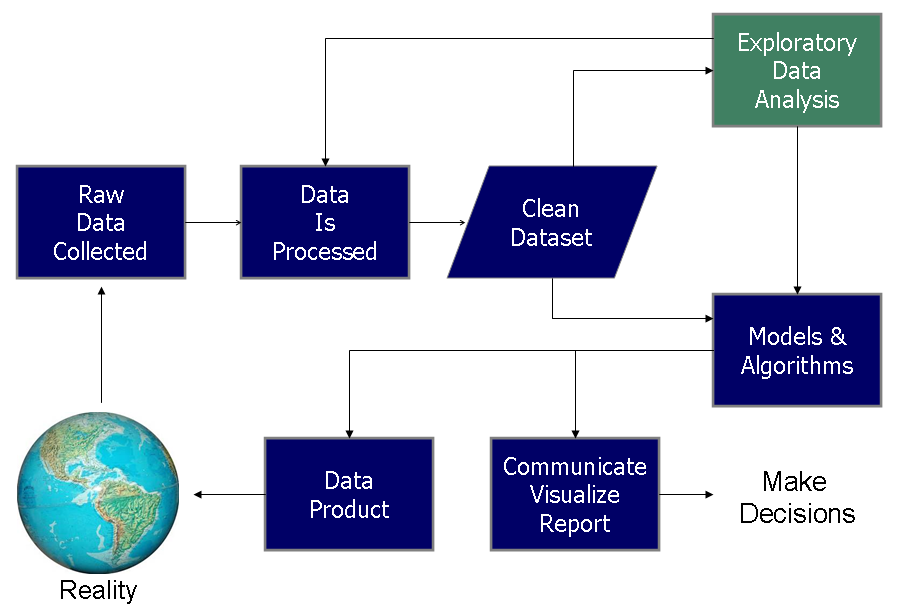
\includegraphics[height=0.85\textheight]{data_science_process}
	\end{figure}
\end{frame}

%------------------------------------------------

\begin{frame}
	\frametitle{Data science process}
	% The structure of the notebook shall follow the Data Science process seen during the lab sessions.
	\begin{enumerate}
		\define{Data acquisition} from the web, a database, a flat file, etc. This includes cleaning the data.
		\vfill
		\define{Data exploration} some exploratory analysis to describe properties of the data and understand the content.
		\vfill
		\define{Data exploitation} use the data to solve a task, to infer knowledge, to draw conclusions.
			The concepts or algorithms taught in class must be used.
		\vfill
		\define{Conclusion} discuss the results and summarize your findings. What did we learn from the data and the project?
	\end{enumerate}
\end{frame}

%------------------------------------------------

\begin{frame}
	\frametitle{Example projects from 2017}
	\begin{figure}
		\centering
		\begin{subfigure}[b]{0.47\linewidth}
			
\includegraphics[width=\linewidth]{project2017_brain}
		\end{subfigure}
		\hfill
		\begin{subfigure}[b]{0.47\linewidth}
			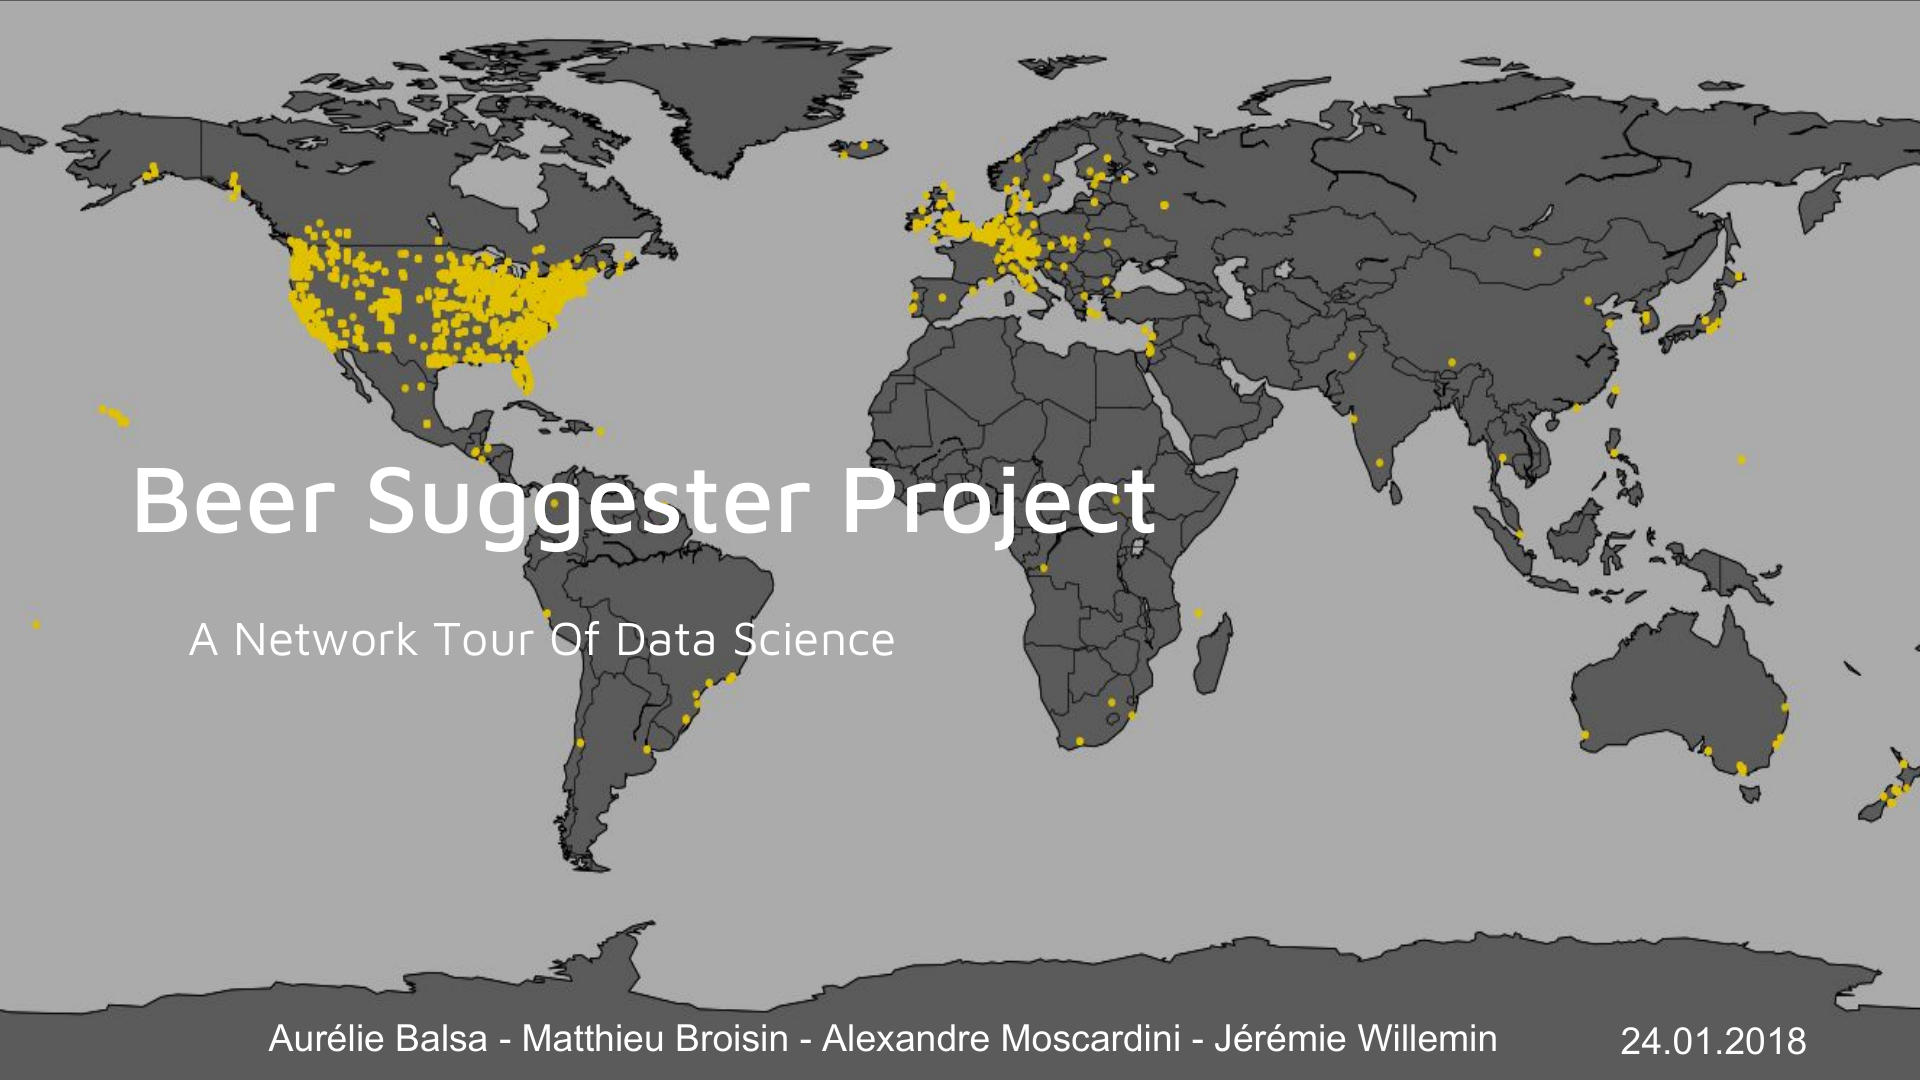
\includegraphics[width=\linewidth]{project2017_beer}
		\end{subfigure}
		\\
		\vspace{0.5em}
		\begin{subfigure}[b]{0.47\linewidth}
			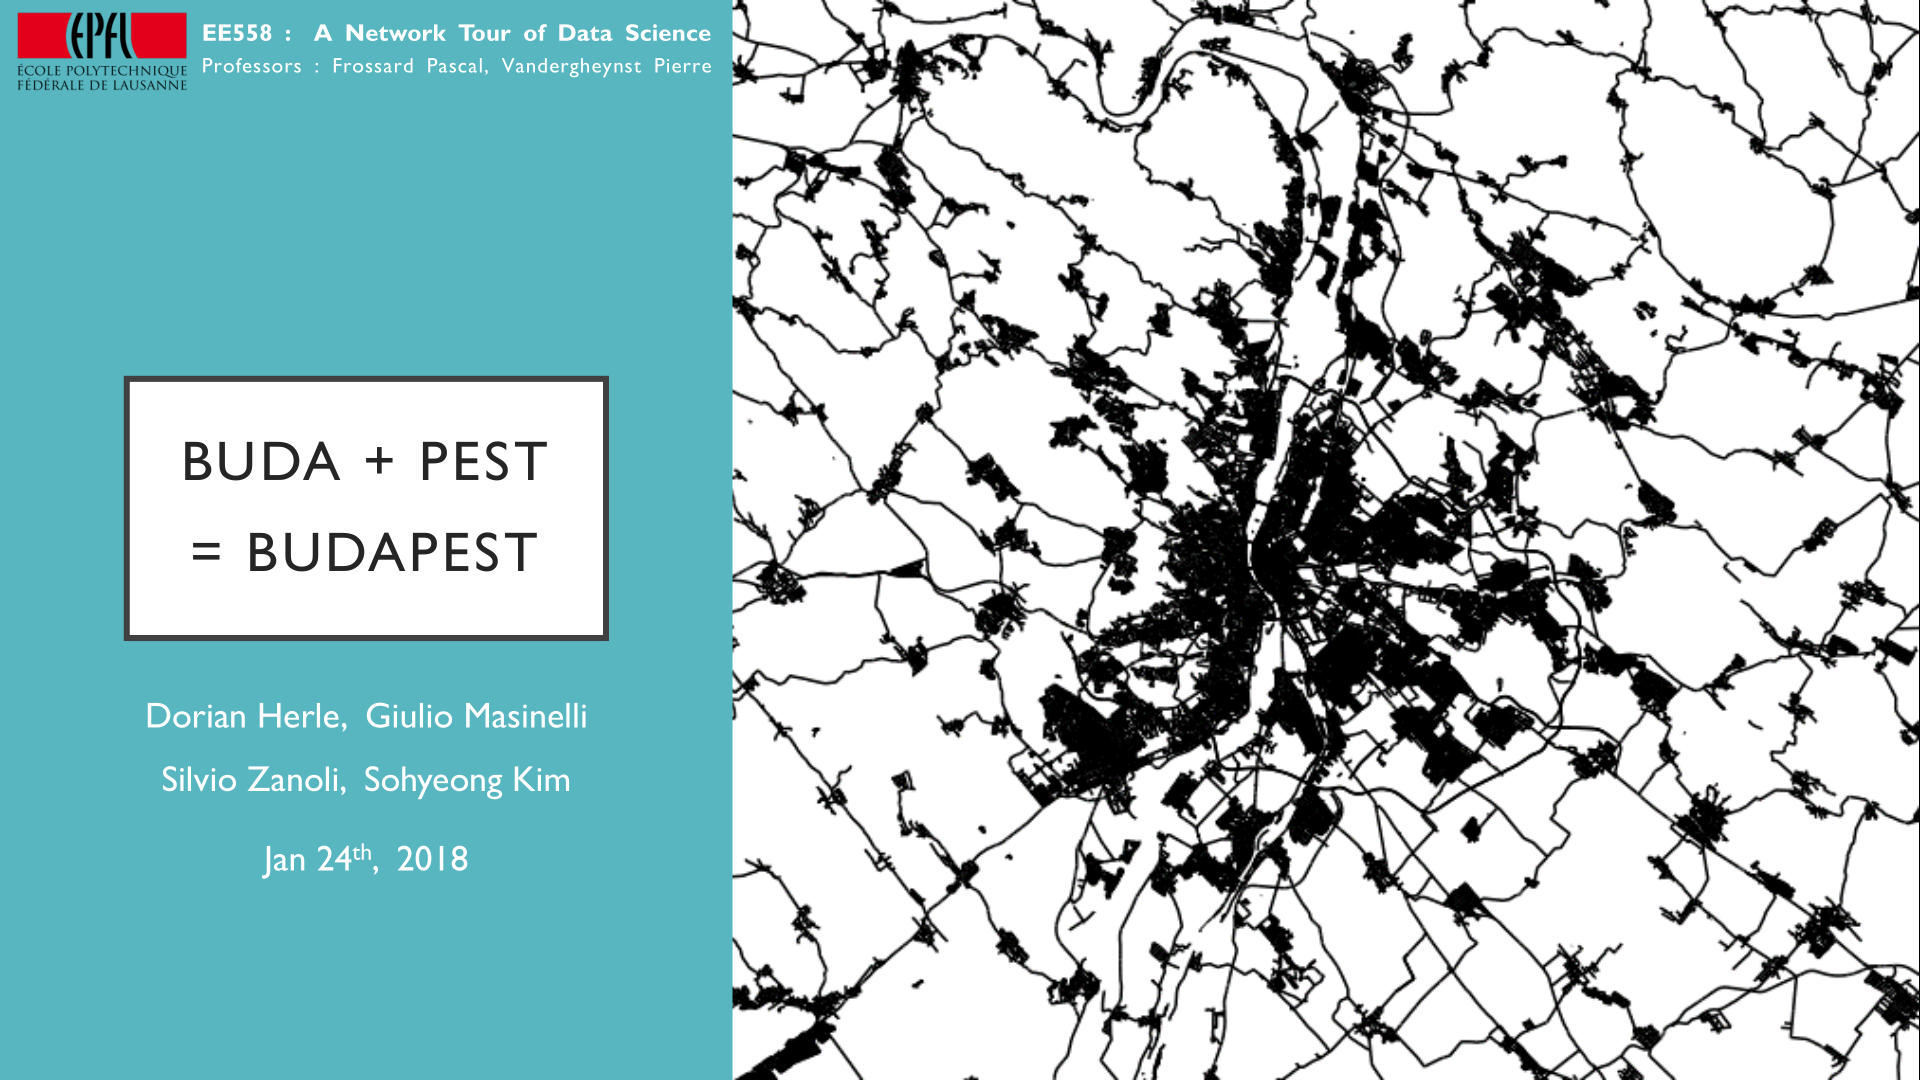
\includegraphics[width=\linewidth]{project2017_roads}
		\end{subfigure}
		\hfill
		\begin{subfigure}[b]{0.47\linewidth}
			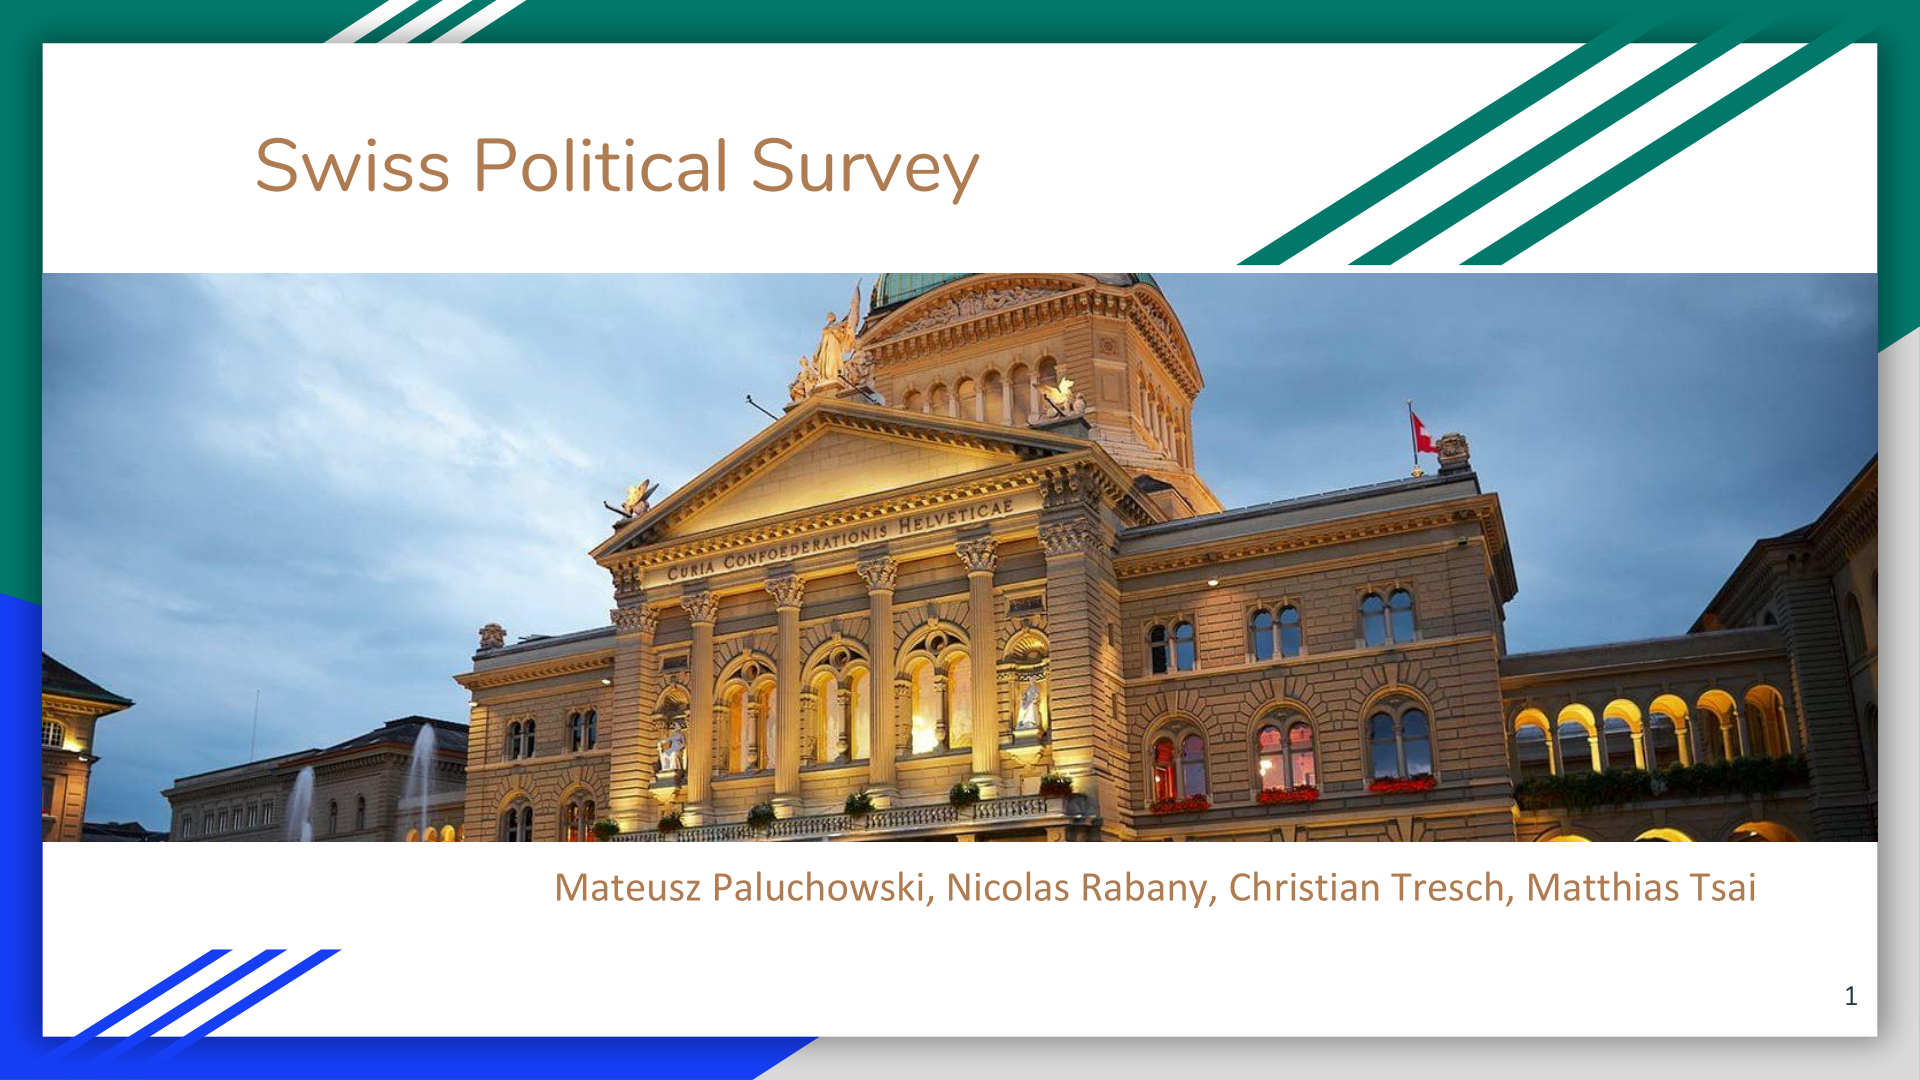
\includegraphics[width=\linewidth]{project2017_politics}
		\end{subfigure}
	\end{figure}
\end{frame}

%------------------------------------------------

\begin{frame}
	\frametitle{Example projects from 2017}
	\begin{figure}
		\centering
		\begin{subfigure}[b]{0.47\linewidth}
			
\includegraphics[width=\linewidth]{project2017_stackoverflow}
		\end{subfigure}
		\hfill
		\begin{subfigure}[b]{0.47\linewidth}
			
\includegraphics[width=\linewidth]{project2017_springs}
		\end{subfigure}
		\\
		\vspace{0.5em}
		\begin{subfigure}[b]{0.47\linewidth}
			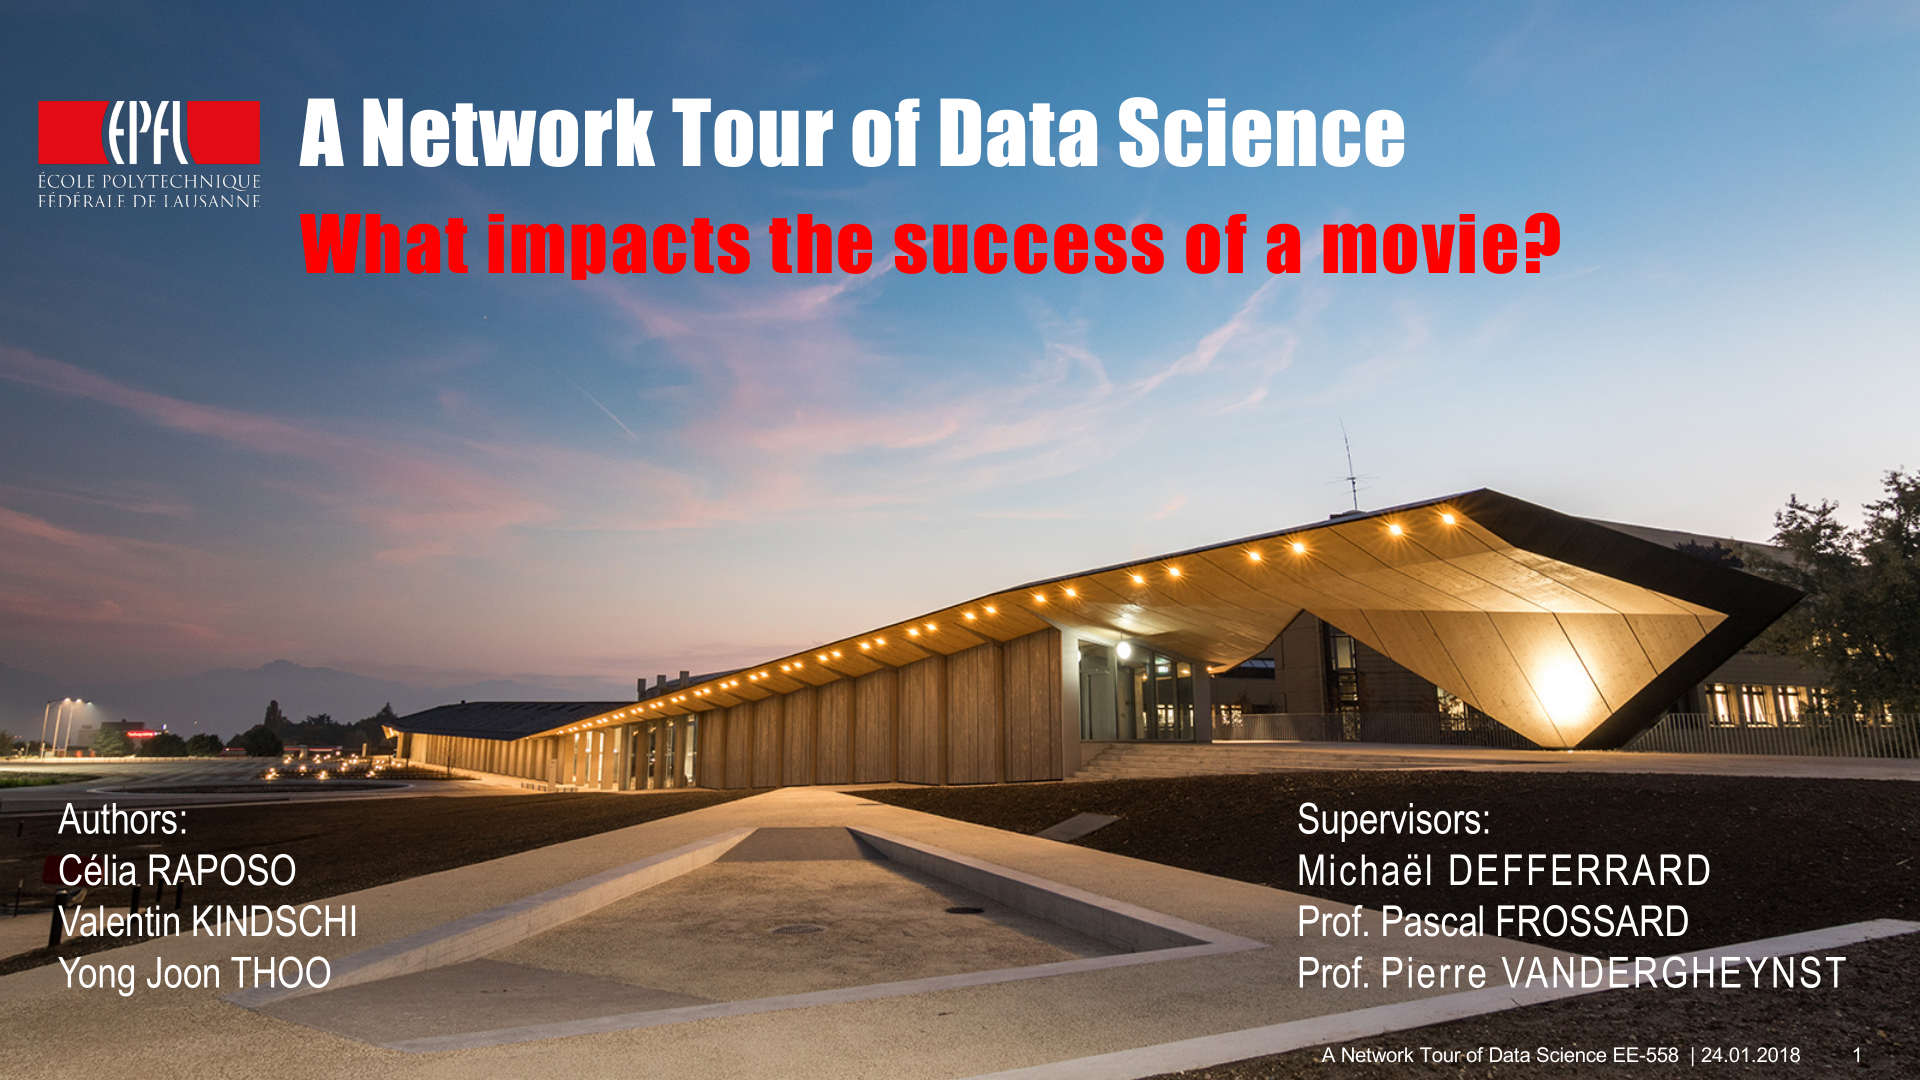
\includegraphics[width=\linewidth]{project2017_movies}
		\end{subfigure}
		\hfill
		\begin{subfigure}[b]{0.47\linewidth}
			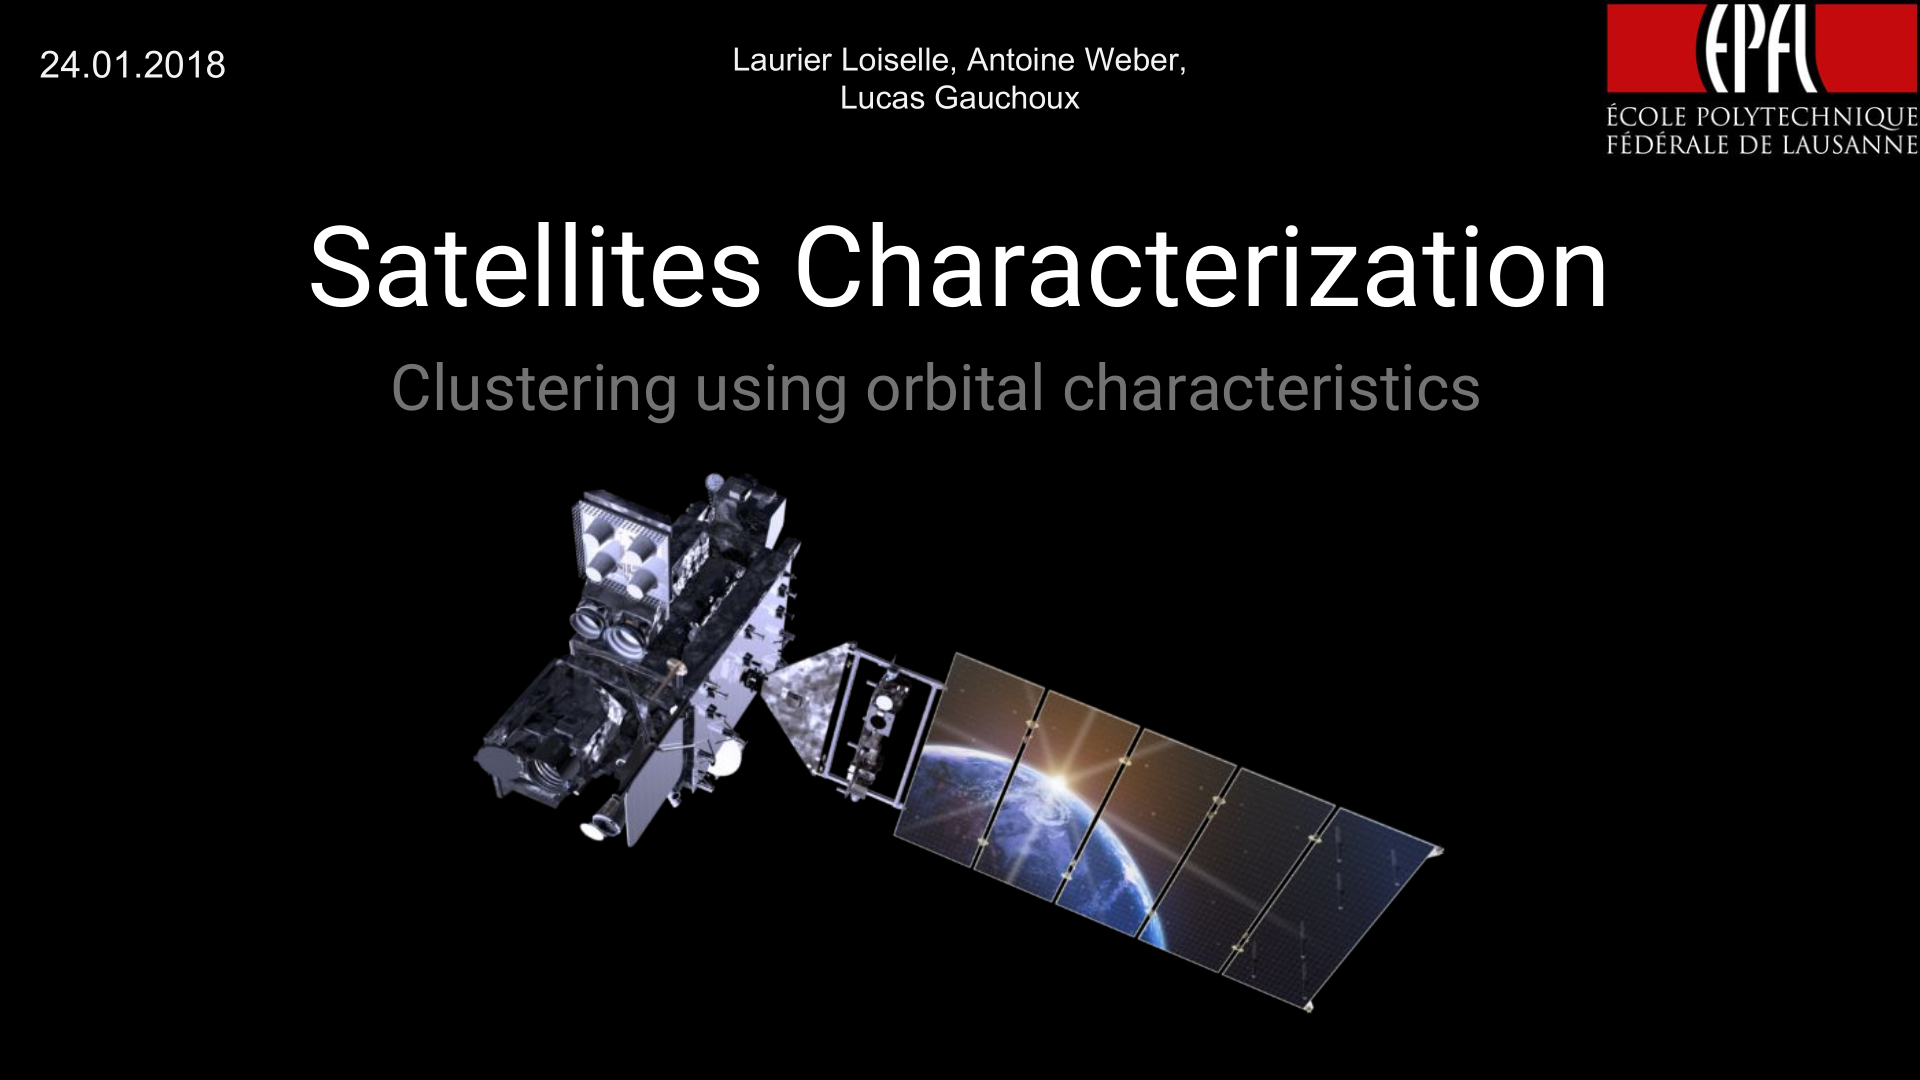
\includegraphics[width=\linewidth]{project2017_satellites}
		\end{subfigure}
	\end{figure}
\end{frame}

%------------------------------------------------

\begin{frame}
	\frametitle{Proposed projects}
	\begin{itemize}
		\item Free Music Archive
		\vfill
		\item US Senators
		\vfill
		\item Wikipedia
		\vfill
		\item Researchers on Twitter
		\vfill
		\item Scientific co-Authorship
		\vfill
		\item Spammers on Social Networks
		\vfill
		\item Citation Network
		\vfill
		\item Terrorist Attacks and Relations
		\vfill
		\item IMDb Films and Crews
		\vfill
		\item Flight Routes
	\end{itemize}
\end{frame}

%------------------------------------------------

\begin{frame}
	\frametitle{Rules}
	\begin{itemize}
		\item Form groups of 4 students. No less, no more.
			\begin{itemize}
				\item One member of the group uploads the deliverables.
				\item The names of all members should appear clearly.
			\end{itemize}
		\vfill
		\item Projects should use tools and ideas from the lectures. While the second part is quite free, it should include graph and network data aspects, and more generally fall under the scope of the class.
		\vfill
		\item The project should follow the data acquisition, exploration and exploitation workflow.
		\vfill
		\item Each member of a team shall contribute equally to the project.
	\end{itemize}
\end{frame}

%------------------------------------------------

\begin{frame}
	\frametitle{Online}
	Moodle: \url{https://moodle.epfl.ch/course/view.php?id=15299}
	\begin{itemize}
		\item slides
		\item grades
		\item official announcements
		\item discussion forum
	\end{itemize}
	\vspace{1em}
	GitHub: \url{https://github.com/mdeff/ntds_2018}
	\begin{itemize}
		\item installation instructions
		\item tutorials
		\item milestones
		\item projects
	\end{itemize}
	\vfill
	\begin{center}
		\Huge Questions?
	\end{center}
\end{frame}

%------------------------------------------------

\end{document}
